\documentclass[12pt,a4paper]{article}
\newcommand{\LabNumber}{4}
\newcommand{\LabTitle}{Cifruri bloc. Algoritmul DES\\ (Sarcina 2.11)}
\newcommand{\LabTitleShort}{Lucrarea de laborator nr. 4 — Criptografie \& Securitate Informațională}
% ---------------------------------------------------------------------------
% Common preamble for the CS laboratory reports (compile with XeLaTeX)
% Strunga Daniel-Ioan, FAF-242 — https://github.com/don09dandidi/CS
% ---------------------------------------------------------------------------
\usepackage{fontspec}
\setmainfont{Latin Modern Roman}
\setsansfont{Latin Modern Sans}
\setmonofont{DejaVu Sans Mono}[Scale=0.85]
\usepackage[english]{babel}
\babelprovide[import, main]{romanian}
\usepackage[a4paper, margin=2.5cm, headheight=15pt]{geometry}
\usepackage{amsmath, amssymb}
\usepackage{booktabs, array, longtable, tabularx}
\usepackage{xcolor}
\usepackage{listings}
\usepackage{fvextra}
\usepackage[most]{tcolorbox}
\usepackage{fancyhdr}
\usepackage{tikz}
\usetikzlibrary{arrows.meta, positioning, shapes.geometric, fit, calc}
\usepackage{enumitem}
\usepackage{caption}
\usepackage{float}
\usepackage[hidelinks]{hyperref}
\usepackage{url}

\definecolor{codebg}{RGB}{248,248,250}
\definecolor{codeframe}{RGB}{200,200,210}
\definecolor{kw}{RGB}{0,0,160}
\definecolor{cmt}{RGB}{0,120,0}
\definecolor{str}{RGB}{160,30,30}
\definecolor{termbg}{RGB}{30,32,40}
\definecolor{termfg}{RGB}{225,228,235}
\definecolor{termbar}{RGB}{60,63,75}
\definecolor{boxblue}{RGB}{230,238,250}

\lstdefinestyle{py}{
  language=Python, basicstyle=\ttfamily\small, backgroundcolor=\color{codebg},
  frame=single, rulecolor=\color{codeframe}, numbers=left, numberstyle=\tiny\color{gray},
  keywordstyle=\color{kw}\bfseries, commentstyle=\color{cmt}\itshape, stringstyle=\color{str},
  breaklines=true, showstringspaces=false, columns=fullflexible, keepspaces=true, tabsize=4,
  extendedchars=true, inputencoding=utf8
}
\lstdefinestyle{sh}{
  language=bash, basicstyle=\ttfamily\small, backgroundcolor=\color{codebg},
  frame=single, rulecolor=\color{codeframe}, numbers=left, numberstyle=\tiny\color{gray},
  keywordstyle=\color{kw}\bfseries, commentstyle=\color{cmt}\itshape, stringstyle=\color{str},
  breaklines=true, showstringspaces=false, columns=fullflexible, keepspaces=true
}
\lstdefinestyle{wl}{
  basicstyle=\ttfamily\small, backgroundcolor=\color{codebg},
  frame=single, rulecolor=\color{codeframe}, numbers=left, numberstyle=\tiny\color{gray},
  morekeywords={RandomPrime,RandomInteger,PowerMod,Mod,GCD,FromDigits,IntegerDigits,
    ToCharacterCode,FromCharacterCode,IntegerLength,BitLength,Module,Print,Hash,Length},
  keywordstyle=\color{kw}\bfseries, commentstyle=\color{cmt}\itshape,
  morecomment=[s]{(*}{*)}, breaklines=true, columns=fullflexible, keepspaces=true
}

% Console session box (as in the Lab 2 report)
\newtcolorbox{terminal}[1][Sesiune Terminal Consolă]{
  enhanced, breakable, colback=termbg, colframe=termbar, coltext=termfg,
  fonttitle=\small\ttfamily\bfseries, title={\textbullet\textbullet\textbullet\quad #1},
  left=4pt, right=4pt, top=2pt, bottom=2pt, boxrule=0.6pt, arc=2pt
}
\DefineVerbatimEnvironment{termout}{Verbatim}{fontsize=\scriptsize, breaklines=true, breakanywhere=true}

\newtcolorbox{infobox}[1]{
  enhanced, breakable, colback=boxblue, colframe=kw!60, fonttitle=\bfseries,
  title={#1}, boxrule=0.6pt, arc=2pt
}

\newcommand{\bignum}[1]{\par\nobreak\vspace{1pt}{\noindent\ttfamily\footnotesize\seqsplit{#1}\par}\vspace{5pt}}
\usepackage{seqsplit}

\pagestyle{fancy}
\fancyhf{}
\renewcommand{\headrulewidth}{0.4pt}
\fancyhead[L]{\footnotesize\textit{\LabTitleShort}}
\fancyhead[R]{\footnotesize strunga.daniel-ioan}
\fancyfoot[C]{\thepage}

\newcommand{\makereporttitle}{%
\begin{titlepage}
  \centering
  {\large\bfseries UNIVERSITATEA TEHNICĂ A MOLDOVEI\par}
  \vspace{2pt}
  {\normalsize Facultatea Calculatoare, Informatică și Microelectronică\par}
  {\normalsize Departamentul Ingineria Software și Automatică\par}
  \vspace{5cm}
  {\LARGE\bfseries LUCRAREA DE LABORATOR NR. \LabNumber\par}
  \vspace{8pt}
  {\Large\bfseries \LabTitle\par}
  \vspace{10pt}
  {\normalsize Disciplina: Criptografie și Securitate Informațională\par}
  \vfill
  \begin{tabular*}{\textwidth}{@{}l@{\extracolsep{\fill}}r@{}}
    \textbf{Autor:} & \textbf{Verificat de:} \\
    Daniel-Ioan Strunga & Lector / Supervizor \\
    Student gr. FAF-242 & Maia Zaica \\
  \end{tabular*}
  \vspace{3cm}

  {\normalsize Chișinău — 2026\par}
\end{titlepage}
}


\begin{document}
\makereporttitle
\tableofcontents
\newpage

\section{Introduction and Laboratory Objectives}
The \textbf{Data Encryption Standard} (DES), published as FIPS~46 in 1977 and reaffirmed as
FIPS~46-3 in 1999, is a symmetric block cipher derived from IBM's Lucifer. It encrypts 64-bit
blocks under a 64-bit key (56 effective bits + 8 parity bits) using a 16-round Feistel network.
Although its key length makes it insecure today (exhaustive search took 22 hours in 1999), DES is
the archetype of modern block ciphers and Triple-DES is still found in legacy systems.

The task number is computed as $\text{nr\_sarcina} = n \bmod 11$ where $n=22$ is the student's
number in the group list: $22 \bmod 11 = 0$, which corresponds to the \textbf{11th} task of the
list, \textbf{Task 2.11}:
\begin{infobox}{Task 2.11}
When encrypting a block with DES, the values $L_{16}$ (32 bits) and $R_{16}$ (32 bits) were obtained.
Determine the encrypted block of the message, represented in hexadecimal.
\end{infobox}

Objectives:
\begin{enumerate}
  \item Study the structure of DES (FIPS 46-3): initial permutation, key schedule, round function,
        S-boxes and final permutation.
  \item Implement a program that solves Task~2.11, showing all the tables used and every
        intermediate step; the input must be entered by the user or generated randomly.
  \item Validate the implementation against known DES test vectors and against OpenSSL.
\end{enumerate}

\section{Theoretical Foundations}
\subsection{General Structure of DES}
\begin{figure}[H]
\centering
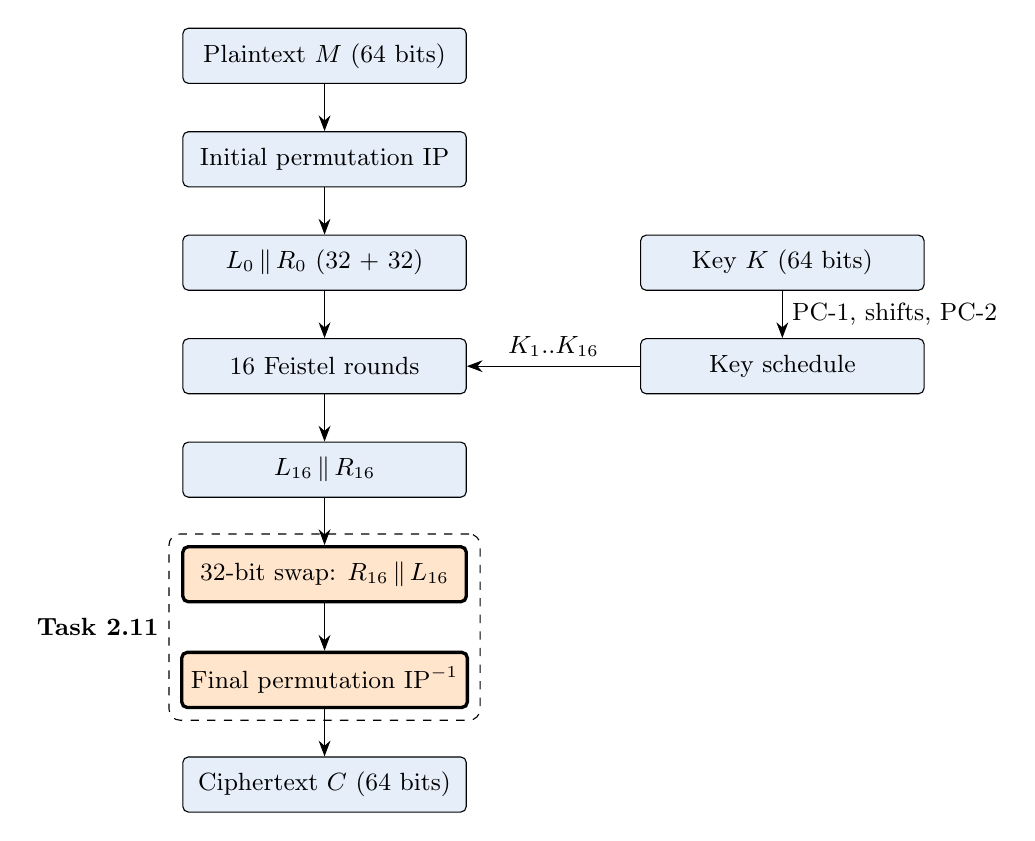
\begin{tikzpicture}[node distance=6mm, every node/.style={font=\small},
  box/.style={draw, rounded corners=2pt, minimum width=36mm, minimum height=7mm, fill=boxblue},
  hl/.style={draw, very thick, rounded corners=2pt, minimum width=36mm, minimum height=7mm, fill=orange!20},
  ar/.style={-{Stealth[length=2mm]}}]
\node[box] (m) {Plaintext $M$ (64 bits)};
\node[box, below=of m] (ip) {Initial permutation IP};
\node[box, below=of ip] (lr) {$L_0 \,\|\, R_0$ (32 + 32)};
\node[box, below=of lr] (r) {16 Feistel rounds};
\node[box, below=of r] (o) {$L_{16} \,\|\, R_{16}$};
\node[hl, below=of o] (sw) {32-bit swap: $R_{16}\,\|\,L_{16}$};
\node[hl, below=of sw] (fp) {Final permutation IP$^{-1}$};
\node[box, below=of fp] (c) {Ciphertext $C$ (64 bits)};
\foreach \a/\b in {m/ip, ip/lr, lr/r, r/o, o/sw, sw/fp, fp/c} \draw[ar] (\a) -- (\b);
\node[box, right=22mm of r] (ks) {Key schedule};
\node[box, above=of ks] (k) {Key $K$ (64 bits)};
\draw[ar] (k) -- node[right]{PC-1, shifts, PC-2} (ks);
\draw[ar] (ks) -- node[above]{$K_1..K_{16}$} (r);
\node[draw, dashed, rounded corners, fit=(sw)(fp), inner sep=4pt, label={[font=\small\bfseries]left:Task 2.11}] {};
\end{tikzpicture}
\caption{Encryption of one 64-bit block with DES; the highlighted steps form Task 2.11}
\end{figure}

\paragraph{Initial permutation.} The 64-bit block is permuted with IP and split into the left
half $L_0$ and the right half $R_0$.

\paragraph{Rounds.} For $i=1,\dots,16$:
\begin{equation}
  L_i = R_{i-1}, \qquad R_i = L_{i-1} \oplus f(R_{i-1}, K_i).
\end{equation}
The round function expands $R_{i-1}$ from 32 to 48 bits with the table $E$, XORs it with the
48-bit round key, splits the result into eight 6-bit groups $B_1\dots B_8$, substitutes each with
the S-box $S_j$ (outer bits select the row, inner 4 bits the column) and finally permutes the
32-bit result with $P$:
\begin{equation}
  f(R,K)=P\big(S_1(B_1)\,S_2(B_2)\cdots S_8(B_8)\big), \qquad B_1\cdots B_8 = E(R)\oplus K.
\end{equation}

\paragraph{Key schedule.} PC-1 drops the 8 parity bits and permutes the key into $K^+$ (56 bits),
split into $C_0$ and $D_0$ (28 bits each). Each round rotates $C$ and $D$ to the left by 1 or 2
positions (shifts \texttt{1,1,2,2,2,2,2,2,1,2,2,2,2,2,2,1}) and PC-2 selects 48 bits forming $K_i$.

\paragraph{Output.} After round 16 the two halves are \emph{not} swapped (equivalently, the swap of
the last round is undone), so the pre-output block is $R_{16}L_{16}$, to which the final permutation
is applied:
\begin{equation}
  C = \mathrm{IP}^{-1}(R_{16}\,\|\,L_{16}). \label{eq:out}
\end{equation}
This makes decryption identical to encryption with the round keys in reverse order.

\subsection{The Final Permutation IP$^{-1}$}
Bit number $i$ of the output is bit number $\mathrm{IP}^{-1}[i]$ of the input $R_{16}L_{16}$
(Table~\ref{tab:ipinv}). IP$^{-1}$ is the inverse of IP: $\mathrm{IP}^{-1}(\mathrm{IP}(x))=x$.

\begin{table}[H]
\centering
\caption{Final permutation IP$^{-1}$ (FIPS 46-3)}
\label{tab:ipinv}
\begin{tabular}{*{8}{c}}
\toprule
40 & 8 & 48 & 16 & 56 & 24 & 64 & 32 \\
39 & 7 & 47 & 15 & 55 & 23 & 63 & 31 \\
38 & 6 & 46 & 14 & 54 & 22 & 62 & 30 \\
37 & 5 & 45 & 13 & 53 & 21 & 61 & 29 \\
36 & 4 & 44 & 12 & 52 & 20 & 60 & 28 \\
35 & 3 & 43 & 11 & 51 & 19 & 59 & 27 \\
34 & 2 & 42 & 10 & 50 & 18 & 58 & 26 \\
33 & 1 & 41 & 9 & 49 & 17 & 57 & 25 \\
\bottomrule
\end{tabular}
\end{table}

A useful observation: the bits of $R_{16}$ (positions 1–32) land on the even output positions and
the bits of $L_{16}$ (positions 33–64) on the odd output positions; e.g.\ output byte~1 is formed by
bits $40,8,48,16,56,24,64,32$ of $R_{16}L_{16}$.

\section{Architecture of the Python Application}
\begin{infobox}{Application Component Structure (\texttt{lab4/des\_task\_2\_11.py})}
\begin{itemize}[leftmargin=*]
  \item \textbf{Tables:} \texttt{IP}, \texttt{IP\_INV}, \texttt{E}, \texttt{P}, \texttt{PC1},
        \texttt{PC2}, \texttt{SHIFTS} and the eight S-boxes, copied from FIPS 46-3.
  \item \textbf{Bit utilities:} \texttt{permute}, \texttt{xor}, \texttt{rotl},
        \texttt{hex\_to\_bits}, \texttt{bits\_to\_hex} working on strings of \texttt{0}/\texttt{1}
        so that every intermediate value can be displayed.
  \item \textbf{Task 2.11:} \texttt{task\_2\_11(L16, R16)} builds $R_{16}L_{16}$, prints the
        bit positions and the IP$^{-1}$ table, shows the origin of every output bit and the
        resulting hexadecimal block.
  \item \textbf{Full DES (verification):} \texttt{round\_keys}, \texttt{feistel},
        \texttt{des\_rounds} compute $L_{16}$, $R_{16}$ for a message and a key, so the result of
        Task~2.11 can be checked against a complete DES encryption.
  \item \textbf{Input modes:} manual entry (8 hex digits or 32 bits per half), random generation,
        or derivation from an 8-character message and key; a self-test runs at start-up.
\end{itemize}
\end{infobox}

\begin{lstlisting}[style=py, caption={Solving Task 2.11 (core logic)}]
def permute(bits: str, table) -> str:
    return "".join(bits[i - 1] for i in table)

def task_2_11(l16: str, r16: str) -> str:
    pre = r16 + l16                 # no swap after round 16 -> R16 || L16
    out = permute(pre, IP_INV)      # final permutation IP^-1
    return bits_to_hex(out)         # 64-bit block in hexadecimal
\end{lstlisting}

\begin{lstlisting}[style=py, caption={Full DES used for verification}]
def feistel(r: str, k: str) -> str:
    x = xor(permute(r, E), k)                     # E(R) xor K_i  (48 bits)
    out = ""
    for j in range(8):
        b = x[6 * j:6 * j + 6]
        row, col = int(b[0] + b[5], 2), int(b[1:5], 2)
        out += format(S_BOXES[j][row][col], "04b")
    return permute(out, P)

def des_rounds(block64: str, key64: str):
    ip = permute(block64, IP)
    l, r = ip[:32], ip[32:]
    for k in round_keys(key64):
        l, r = r, xor(l, feistel(r, k))
    return l, r                                   # (L16, R16)
\end{lstlisting}

\section{Results}
\subsection{Validation on the Reference Test Vector}
The classic example of J.\ Orlin Grabbe (\emph{The DES Algorithm Illustrated}) uses
$M=$ \texttt{0123456789ABCDEF} and $K=$ \texttt{133457799BBCDFF1} and obtains
$L_{16}=$ \texttt{43423234}, $R_{16}=$ \texttt{0A4CD995}. The program reproduces these values and
the expected ciphertext:
\begin{terminal}
\begin{termout}
$ python3 des_task_2_11.py --values 43423234 0A4CD995
  [OK] Autotest DES: vectorii de test cunoscuți sunt reproduși corect.
  ...
  Pasul 3. Rezultatul
    C (binar) = 10000101 11101000 00010011 01010100 00001111 00001010 10110100 00000101
    C (hex)   = 85E813540F0AB405
\end{termout}
\end{terminal}

\subsection{Worked Example: Message ``Strunga '' with Key ``FAF-242!''}
To obtain realistic $L_{16}$, $R_{16}$ the message \texttt{"Strunga\textvisiblespace"}
(hex \texttt{537472756E676120}) was encrypted with the key \texttt{"FAF-242!"}
(hex \texttt{4641462D32343221}). The 16 rounds computed by the program are:

\begin{table}[H]
\centering
\caption{Round keys and halves for $M$ = \texttt{537472756E676120}, $K$ = \texttt{4641462D32343221}}
\small
\begin{tabular}{cccc|cccc}
\toprule
$i$ & $K_i$ & $L_i$ & $R_i$ & $i$ & $K_i$ & $L_i$ & $R_i$ \\
\midrule
1 & \texttt{C084AEA13002} & \texttt{00FE1035} & \texttt{06727476} & 9  & \texttt{2F430B4C4482} & \texttt{370E05B8} & \texttt{3AC24CB8} \\
2 & \texttt{D086A21B0391} & \texttt{06727476} & \texttt{B001119F} & 10 & \texttt{2B1189CC4049} & \texttt{3AC24CB8} & \texttt{15B4A83A} \\
3 & \texttt{F09A22134101} & \texttt{B001119F} & \texttt{7D82B3BD} & 11 & \texttt{1908D982D248} & \texttt{15B4A83A} & \texttt{AC1394CB} \\
4 & \texttt{A0B246422104} & \texttt{7D82B3BD} & \texttt{9E11D0C3} & 12 & \texttt{156898909720} & \texttt{AC1394CB} & \texttt{22711FE9} \\
5 & \texttt{205656E0218C} & \texttt{9E11D0C3} & \texttt{FAA48AB9} & 13 & \texttt{162D84980E20} & \texttt{22711FE9} & \texttt{FA987260} \\
6 & \texttt{64517060128B} & \texttt{FAA48AB9} & \texttt{96B7A8B6} & 14 & \texttt{5A2C05586A10} & \texttt{FA987260} & \texttt{D9DD88C4} \\
7 & \texttt{86C17156102B} & \texttt{96B7A8B6} & \texttt{3850FDD3} & 15 & \texttt{49A42C316018} & \texttt{D9DD88C4} & \texttt{942CA100} \\
8 & \texttt{8F4313061968} & \texttt{3850FDD3} & \texttt{370E05B8} & 16 & \texttt{C1A4AC820E95} & \texttt{942CA100} & \texttt{48F295CB} \\
\bottomrule
\end{tabular}
\end{table}

Hence the input of Task 2.11 is $L_{16}=$ \texttt{942CA100}, $R_{16}=$ \texttt{48F295CB}.

\paragraph{Step 1 — pre-output block.}
\begin{center}\small
$R_{16}L_{16} =$ \texttt{01001000 11110010 10010101 11001011 10010100 00101100 10100001 00000000}
\end{center}

\paragraph{Step 2 — final permutation.} Each output bit $c_i$ takes bit $b_{\mathrm{IP}^{-1}[i]}$
of $R_{16}L_{16}$:
\begin{table}[H]
\centering
\caption{Application of IP$^{-1}$ to $R_{16}L_{16}$, byte by byte}
\begin{tabular}{clcc}
\toprule
Byte & Source positions in $R_{16}L_{16}$ (from IP$^{-1}$) & Bits & Hex \\
\midrule
1 & 40, 8, 48, 16, 56, 24, 64, 32 & \texttt{00001101} & \texttt{0D} \\
2 & 39, 7, 47, 15, 55, 23, 63, 31 & \texttt{00010001} & \texttt{11} \\
3 & 38, 6, 46, 14, 54, 22, 62, 30 & \texttt{10100100} & \texttt{A4} \\
4 & 37, 5, 45, 13, 53, 21, 61, 29 & \texttt{01100001} & \texttt{61} \\
5 & 36, 4, 44, 12, 52, 20, 60, 28 & \texttt{10010100} & \texttt{94} \\
6 & 35, 3, 43, 11, 51, 19, 59, 27 & \texttt{00111000} & \texttt{38} \\
7 & 34, 2, 42, 10, 50, 18, 58, 26 & \texttt{01010001} & \texttt{51} \\
8 & 33, 1, 41, 9, 49, 17, 57, 25 & \texttt{10011101} & \texttt{9D} \\
\bottomrule
\end{tabular}
\end{table}

\paragraph{Step 3 — result.}
\[
\boxed{C = \texttt{0D11A4619438519D}}
\]
The program checks the result against a full DES encryption, and the same value is returned by
OpenSSL:
\begin{terminal}
\begin{termout}
$ printf 'Strunga ' | openssl enc -des-ecb -K 4641462D32343221 -nopad \
      -provider legacy -provider default | od -An -tx1
 0d 11 a4 61 94 38 51 9d
\end{termout}
\end{terminal}

\subsection{Random Input Mode}
With \texttt{--random} (or option 2 in the menu) $L_{16}$ and $R_{16}$ are generated with the
cryptographically secure generator \texttt{secrets.randbits(32)} and the same steps are printed.

\section{Source Code and Repository}
\begin{center}
\url{https://github.com/don09dandidi/CS} \quad (directory \texttt{lab4/})
\end{center}

\subsection{Build and Execution Instructions}
\begin{lstlisting}[style=sh]
git clone https://github.com/don09dandidi/CS.git
cd CS/lab4
python3 des_task_2_11.py                          # interactive menu
python3 des_task_2_11.py --values 942CA100 48F295CB # L16, R16 given in hex
python3 des_task_2_11.py --random                  # random L16, R16
python3 des_task_2_11.py --from-message "Strunga " "FAF-242!"
\end{lstlisting}

\section{Conclusion}
\begin{enumerate}
  \item \textbf{Final stage of DES:} the ciphertext is obtained from the last round output by
        concatenating the halves in reversed order, $R_{16}L_{16}$, and applying the final
        permutation IP$^{-1}$; for $L_{16}=$ \texttt{942CA100}, $R_{16}=$ \texttt{48F295CB} the
        block is \texttt{0D11A4619438519D}.
  \item \textbf{Why the swap is omitted:} omitting the swap after round 16 and using IP$^{-1}$ makes
        the Feistel network self-inverse, so the same circuit decrypts when the round keys are
        applied in the order $K_{16},\dots,K_1$.
  \item \textbf{IP and IP$^{-1}$} have no cryptographic strength (they are public and fixed); the
        security of DES comes from the non-linear S-boxes and the 16 rounds of confusion and
        diffusion. The weakness of DES is its 56-bit key ($2^{56}\approx7.2\times10^{16}$ keys).
  \item \textbf{Verification:} the implementation reproduces the reference test vectors
        of Grabbe and FIPS 81 (\texttt{85E813540F0AB405} and
        \texttt{3FA40E8A984D4815}) and agrees with OpenSSL.
\end{enumerate}

\begin{thebibliography}{9}
\bibitem{fips} NIST, \emph{FIPS PUB 46-3: Data Encryption Standard (DES)}, 1999.
\bibitem{grabbe} J.\ Orlin Grabbe, \emph{The DES Algorithm Illustrated}.
\bibitem{stallings} William Stallings, \emph{Cryptography and Network Security: Principles and
  Practice}, 7th Edition, Pearson, 2017.
\bibitem{guide} \emph{Lucrare de laborator nr.~4. Cifruri bloc. Algoritmul DES}, UTM, FCIM, 2026.
\end{thebibliography}
\end{document}
